% chktex-file 1 chktex-file 8

\tikzmath{
\dchamber       = 3;
\lchamber       = 5;
\xchambercenter = \lchamber/2;
\dbarrel        = 1;
\lbarrel        = 5.5;
\lvalve         = 0.5;
\ldead          = 1.5;
\ylowbarrel     = (\dchamber - \dbarrel)/2; 
\yhighbarrel    = \ylowbarrel + \dbarrel;
\xvalvestart    = \lchamber;
\xdeadstart     = \lchamber + \lvalve;
\xbarrelstart   = \lchamber + \lvalve + \ldead;
\xbarrelend     = \lchamber + \lvalve + \ldead + \lbarrel;
\lproj          = 2;
\xproj          = \xbarrelstart + 1;
\ycenter        = \dchamber/2;
\ylbarrel       = \ycenter + (\dchamber + \dbarrel)/4;
\xdead          = \xdeadstart + \ldead/2;
\yxz            = \ycenter - (\dchamber + \dbarrel)/4;
\xdbarrel       = \xbarrelend - 1;
\ymin           = (\ycenter + \ylowbarrel)/2;
}

\begin{figure}
\centering
\begin{tikzpicture}
\draw[thick] (\xbarrelend, \yhighbarrel) -- (\lchamber, \yhighbarrel) -- (\lchamber, \dchamber) -- (0, \dchamber) -- (0, 0)         -- (\lchamber, 0) -- (\lchamber, \ylowbarrel) -- (\xbarrelend, \ylowbarrel);

\draw[thick,dashed] (\lchamber, \ylowbarrel) -- (\lchamber, \yhighbarrel);

\fill[fill=gray,draw=black,thick] (\xproj, \ylowbarrel) rectangle ++(\lproj, \dbarrel) node[pos=0.5] {\small\color{white}projectile};

\fill[fill=gray,draw=black,thick] (\xvalvestart, \ylowbarrel) rectangle ++(\lvalve, \dbarrel) node[pos=0.5, rotate=90] {\small\color{white}valve};

\draw[<->,thick,fill=white] (\xbarrelstart, \ylbarrel) -- node[above] {$l_\text{travel}$} (\xbarrelend, \ylbarrel); % `fill=white` added to make the text fully visible in LaTeXML
\draw[thick,dashed] (\xbarrelend, \yhighbarrel) -- (\xbarrelend, \dchamber);

\node[draw=white] at (\xchambercenter, \ycenter) {$V_\text{chamber}$}; % `draw=white` added to make the text fully visible in LaTeXML
\node[draw=white] at (\xdead, \ycenter) {$V_\text{dead}$}; 

\draw[<->,thick] (\xdeadstart, \ylbarrel) -- node[above] {$x_\text{0}$} (\xbarrelstart, \ylbarrel);
\draw[thick,dashed] (\xdeadstart, \ylowbarrel) -- (\xdeadstart, \dchamber);
\draw[thick,dashed] (\xbarrelstart, \ylowbarrel) -- (\xbarrelstart, \dchamber);

\draw[<->,thick] (\lchamber, \yxz) -- node[below] {$x$} (\xproj, \yxz);
\draw[thick,dashed] (\xproj, 0) -- (\xproj, \ylowbarrel);

\draw[<->,thick] (\xdbarrel, \ylowbarrel) -- node[right] {$d_\text{barrel}$} (\xdbarrel, \yhighbarrel);
\end{tikzpicture}
\caption{Model pneumatic blaster at arbitrary time as represented in BlasterSim.\label{fig:pneumatic arbitrary time}}
\end{figure}

\begin{figure}
\centering
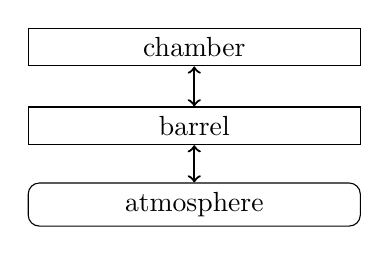
\begin{tikzpicture}
\tikzstyle{cv}       = [rectangle, minimum width=12em, text centered, draw=black]
\tikzstyle{cv_const} = [rectangle, rounded corners, minimum width=12em, text centered, draw=black]
\tikzstyle{arrow}    = [thick, <->]

\node (chamber) [cv]                        {chamber};
\node (barrel)  [cv, below of=chamber]      {barrel};
\node (atm)     [cv_const, below of=barrel] {atmosphere};

\draw [arrow] (chamber) -- (barrel);
\draw [arrow] (barrel)  -- (atm);
\end{tikzpicture}
\caption{Abstract connected control volume view of a pneumatic blaster.\label{fig:pneumatic control volumes}}
\end{figure}
